\documentclass{amsart}
\usepackage{style_reopn}
\begin{document}

%%%%%%%%%%%%%%%%
%%%%%%%%%%%%%%%%
\section{Structured cospans}
\label{sec_structured-cospans}
	
\begin{df} \label{df_structured-cospans}
	Given a functor $ L \from \A \to \X $, a $ L $-structured cospan is a diagram of form $ L a \to x \gets L b $. 
\end{df}
	
\begin{df} \label{df_(-)Csp-category}
	Fix a category $ \X $ and a functor $ L \from \A \to \X $. Denote by $ \FuncCsp{ L } $ the category with objects are those from $ \A $ and with morphisms of type $ a \to b $ are isomorphism classes of $ L $-structured cospans $ La \to x \gets Lb $.
\end{df}

\begin{df} \label{df_StrCsp-category}
	Denote by $ \StrCsp{L} $ the category whose objects are $ L $-open objects and arrows are triples $ (f,g,h) $ that fit into a commuting diagram
	\[
	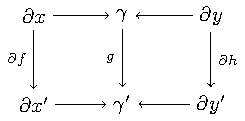
\includegraphics{diag_open-graph-morph_reopn}
	\]
\end{df}

\begin{thm} \label{thm_StrCsp-topos}
	Let $ L \dashv R \from \A \to \X $ be an adjunction between topoi.  Then $ \StrCsp{L} $ is a topos.  
\end{thm}

%%%%%%%%%%%%%%%%
%%%%%%%%%%%%%%%%
\section{Rewriting}

\begin{df} \label{df_adhesive-category}
	A category with pullbacks is \defn{adhesive} if pushouts along monics exist and are \emph{Van Kampen}.
\end{df} 

\begin{thm} \label{thm_topoi-adhesive}
	Topoi are adhesive.
\end{thm}

\begin{cor} \label{thm_category-StrCsp-adhsv}
	Let $ L \dashv R \from \A \to \X $ be an adjunction between topoi.  The category $ \StrCsp{L} $ is adhesive.
\end{cor}

\begin{df} \label{df_rewrite-rule}
	For $ \C $ an adhesive category, an \defn{$ \C $-rewrite rule} (often called a production) is a span $ a \gets b \to c $ inside $ \C $.  When both legs of the span are monic, we say the rewrite rule is \defn{linear}.
\end{df}	
	
\begin{df} \label{df_pushout-complement}
	Given composable arrows $ a \to b \to y $ we say that an arrow $ a \to x $ is a \defn{pushout complement} if it fits into a pushout diagram
	\[
	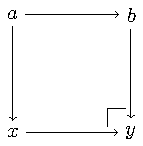
\includegraphics{diag_pushout-complement_reopn}
	\]
\end{df}

\begin{df} \label{df_derived-rewrite-rule}
	Given a $ \C $-rewrite rule $ a \gets b \to c $ and a $ \C $-arrow $a \to x$ such that $ b \to a \to x $ has a pushout complement, a \defn{derived (linear) rewrite rule} is the bottom row of the induced double pushout diagram
	\[
	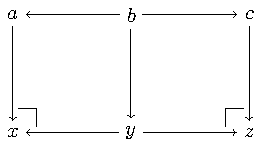
\includegraphics{diag_derived-rewrite-rule}
	\]
\end{df}

\begin{df} \label{df_grammar-and-language}
	A \defn{(linear) grammar} consists of an adhesive category $ \A $ and a set of (linear) $ \A $-rewrite rules.  Observe that $ \A $-rewrite rules are actually arrows in $ \Sp{\A} $.  Given a grammar $ \Gamma $, the subcategory $ \mathcal{L} ( \Gamma ) $ of $ \Sp{ \A } $ generated by the set of rewrites derived from $ \Gamma $ is called a \defn{language}.  
\end{df}

\begin{lem} \label{thm_open-objects-language}
	Let $ (\A , \otimes_{\A} , I_{\A}) $ be a symmetric monoidal category with pullbacks and $ (\X , \otimes_{\X} , I_{\X}) $ be a symmetric monoidal topos.  Let $ L \dashv R \from \A \to \X $ be an adjunction where $ L $ preserves pullbacks.
	
	Fix a grammar $ \Gamma $ in the topos $ \StrCsp{L} $.  The generated  language $ \mathcal{L}(\Gamma) $ is a sub-bicategory of $ \Sp{\StrCsp{L}} $. 
\end{lem}

%%%%%%%%%%%%%%%%
%%%%%%%%%%%%%%%%
\section{Non-linear rewriting of open objects}

\begin{df} \label{df_arrow-category-rewrite}
	Let $ \A $ be a category with pullbacks, $ \X $ be a category with pullbacks and pushouts, and $ L \from \A \to \X $ be a functor preserving pullbacks.  Denote by $ \mathcal{P}(\Sp{\StrCsp{L}}) $ the preorder whose objects are $ L $-open objects and arrows $ (L a \to x \gets L a') \leq (L c \to x \gets L c') $ whenever there is a $ \Sp{\StrCsp{L}} $-arrow with form
	\[
	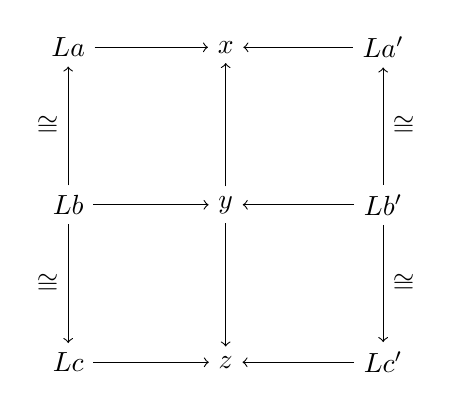
\begin{tikzpicture}
	\node (a) at (-1,1) {$ L a $};
	\node (x) at (1,1) {$ x $};
	\node (a') at (3,1) {$ L a' $};
	\node (b) at (-1,-1) {$ L b $};
	\node (y) at (1,-1) {$ y $};
	\node (b') at (3,-1) {$ L b' $};
	\node (c) at (-1,-3) {$ L c $};
	\node (z) at (1,-3) {$ z $};
	\node (c') at (3,-3) {$ L c' $};
	%
	\draw [->] (a) to (x);
	\draw [->] (a') to (x);
	\draw [->] (b) to (y);
	\draw [->] (b') to (y);
	\draw [->] (c) to (z);
	\draw [->] (c') to (z);
	\draw [->] (b) to node [left] {$ \cong $} (a);
	\draw [->] (b) to node [left] {$ \cong $} (c);
	\draw [->] (y) to (x);
	\draw [->] (y) to (z);
	\draw [->] (b') to node [right] {$ \cong $} (a');
	\draw [->] (b') to node [right] {$ \cong $} (c');
	\end{tikzpicture}
	\]
\end{df}

\begin{df} \label{df_rewrite-dble-cat}
	Let $ \A $ be a category with pullbacks, $ \X $ a category with pullbacks and pushouts, and $ L \from \A \to \X $ be a functor preserving pullbacks.	Define the double category $ \RRewrite{L} $ to have object category $ \core{ \Sp{ \A } } $ and have arrow category $ \C $
	as described in Definition \ref{df_arrow-category-rewrite}.
	
	Alternatively, $ \RRewrite{L} $ is the double category with $ \A $-objects as 0-cells, spans in $ \A $ with isomorphic legs as vertical 1-cells, $ L $-open objects as horizontal 1-cells, and a unique 2-cell if there exists a commuting diagram in $ \X $ of form	
	\[
	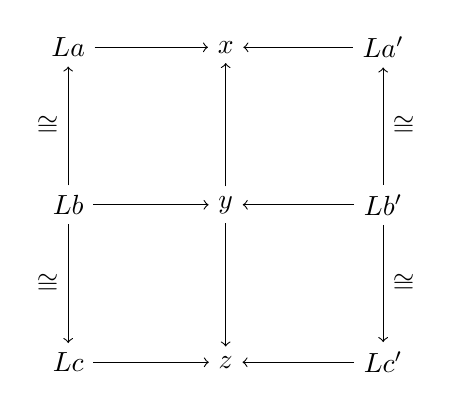
\begin{tikzpicture}
	\node (a) at (-1,1) {$ L a $};
	\node (x) at (1,1) {$ x $};
	\node (a') at (3,1) {$ L a' $};
	\node (b) at (-1,-1) {$ L b $};
	\node (y) at (1,-1) {$ y $};
	\node (b') at (3,-1) {$ L b' $};
	\node (c) at (-1,-3) {$ L c $};
	\node (z) at (1,-3) {$ z $};
	\node (c') at (3,-3) {$ L c' $};
	%
	\draw [->] (a) to (x);
	\draw [->] (a') to (x);
	\draw [->] (b) to (y);
	\draw [->] (b') to (y);
	\draw [->] (c) to (z);
	\draw [->] (c') to (z);
	\draw [->] (b) to node [left] {$ \cong $} (a);
	\draw [->] (b) to node [left] {$ \cong $} (c);
	\draw [->] (y) to (x);
	\draw [->] (y) to (z);
	\draw [->] (b') to node [right] {$ \cong $} (a');
	\draw [->] (b') to node [right] {$ \cong $} (c');
	\end{tikzpicture}
	\]	
\end{df}

\begin{thm} \label{thm_rewrite-isofibrant}
	The double category $ \RRewrite{L} $ is isofibrant.
\end{thm}

\begin{thm} \label{thm_rewrite-dble-cat-smc}
	Let $ (\A, \otimes_{\A}, I_{\A}) $ and $ (\X, \otimes_{\X}, I_{\X}) $ be symmetric monoidal categories so that $ \A $ has a pullbacks and $ \X $ has pullbacks and pushouts. If $ L \from (\A, \otimes_{\A}, I_{\A}) \to (\X, \otimes_{\X}, I_{\X}) $ preserves pullbacks, then $ (\RRewrite{L} , \otimes , I) $ is a symmetric monoidal double category with $ \otimes $ defined by
	\[
	\left( L a \to x \gets L b \right) \otimes
	\left( L c \to y \gets L d	\right) \coloneqq
	L (a \otimes_{\A} c) \to 
	x \otimes_{\X} y \gets L (b \otimes_{\A} d)
	\]
	and $ I $ defined by		
	\[
	I \coloneqq ( L I_{\A} \to I_{\X} \gets L I_{\X} ).
	\]
\end{thm}

\begin{thm} \label{thm_rewrite_smcc}
	Let $ (\A, \otimes_{\A}, I_{\A}) $ and $ (\X, \otimes_{\X}, I_{\X}) $ be symmetric monoidal categories where $ \A $ has pullbacks and $ \X $ has pullbacks and pushouts.  Let $ L \from (\A, \otimes_{\A}, I_{\A}) \to (\X, \otimes_{\X}, I_{\X}) $ be a pullback preserving symmetric monoidal functor.	
	
	The horizontal edge bicategory $ \Rewrite{L} \coloneqq  \mathcal{H} \left( \RRewrite{L} \right) $ in the sense of Shulman is symmetric monoidal. Moreover, if the monoidal products $ \otimes_{\A} $ and $ \otimes_{\X} $ are coproducts, then the symmetric monoidal bicategory $ \Rewrite{L} $ is compact closed.
\end{thm}

\begin{thm} \label{thm_rewrite-bicategory-relations}
	Let $ (\A, \otimes_{\A}, I_{\A}) $ and $ (\X, \otimes_{\X}, I_{\X}) $ be symmetric monoidal categories so that $ \A $ has a pullbacks and $ \X $ has pullbacks and pushouts.  Let $ L \from (\A, \otimes_{\A}, I_{\A}) \to (\X, \otimes_{\X}, I_{\X}) $ be a pullback preserving functor.	
	
	The bicategory $ \Rewrite{L} $ is a bicategory of relations in the sense of Carboni and Walters.
\end{thm}

\begin{thm} \label{thm_}
	Let $ (\A , \otimes_{\A} , I_{\A}) $ be a symmetric monoidal category with pullbacks and $ (\X , \otimes_{\X} , I_{\X}) $ be a symmetric monoidal topos.  Let $ L \dashv R \from \A \to \X $ be an adjunction where $ L $ preserves pullbacks.
	
	Suppose each element from a grammar $ \Gamma $ in $ \StrCsp{L} $ is of the form 
	\[
	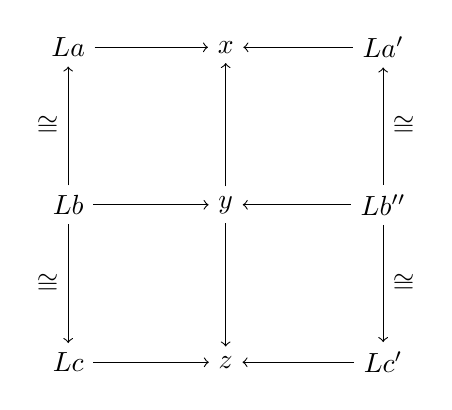
\begin{tikzpicture}
	\node (a) at (-1,1) {$ L a $};
	\node (x) at (1,1) {$ x $};
	\node (a') at (3,1) {$ L a' $};
	\node (b) at (-1,-1) {$ L b $};
	\node (y) at (1,-1) {$ y $};
	\node (b') at (3,-1) {$ L b'' $};
	\node (c) at (-1,-3) {$ L c $};
	\node (z) at (1,-3) {$ z $};
	\node (c') at (3,-3) {$ L c' $};
	%
	\draw [->] (a) to (x);
	\draw [->] (a') to (x);
	\draw [->] (b) to (y);
	\draw [->] (b') to (y);
	\draw [->] (c) to (z);
	\draw [->] (c') to (z);
	\draw [->] (b) to node [left] {$ \cong $} (a);
	\draw [->] (b) to node [left] {$ \cong $} (c);
	\draw [->] (y) to (x);
	\draw [->] (y) to (z);
	\draw [->] (b') to node [right] {$ \cong $} (a');
	\draw [->] (b') to node [right] {$ \cong $} (c');
	\end{tikzpicture}
	\]
	Then $ \Gamma $ generates a sub-double category of $ \RRewrite{L} $ as follows:
	\begin{itemize}
		\item generate the sub-bicategory $ \mathcal{L}(\Gamma)  \subseteq \Sp{\StrCsp{L}} $ as in Lemma \ref{thm_open-objects-language}, 
		\item with $ \mathcal{L}(\Gamma) $, define the subcategory $ \mathcal{P}(\mathcal{L}(\Gamma)) $ as in Definition \ref{df_arrow-category-rewrite},
	\end{itemize}  
	
	Form the category as described in Definition \ref{df:ArrCatRwrt} from $ \mathcal{L}(\Gamma) $. Pair this, as an arrow category, with the object category $ \core{\Sp{\A}} $.  
\end{thm}

\begin{thm}
	If $ \Gamma $ has only elements of the form 
	\[
	\begin{tikzpicture}
	\node (a) at (-1,1) {$ L a $};
	\node (x) at (1,1) {$ x $};
	\node (a') at (3,1) {$ L a' $};
	\node (b) at (-1,-1) {$ L a $};
	\node (y) at (1,-1) {$ y $};
	\node (b') at (3,-1) {$ L a' $};
	\node (c) at (-1,-3) {$ L a $};
	\node (z) at (1,-3) {$ z $};
	\node (c') at (3,-3) {$ L a' $};
	%
	\draw [->] (a) to (x);
	\draw [->] (a') to (x);
	\draw [->] (b) to (y);
	\draw [->] (b') to (y);
	\draw [->] (c) to (z);
	\draw [->] (c') to (z);
	\draw [->] (b) to node [left] {$ = $} (a);
	\draw [->] (b) to node [left] {$ = $} (c);
	\draw [->] (y) to (x);
	\draw [->] (y) to (z);
	\draw [->] (b') to node [right] {$ = $} (a');
	\draw [->] (b') to node [right] {$ = $} (c');
	\end{tikzpicture}
	\]
	then $ \Gamma $ generates a sub-bicategory of $ \Rewrite{L} $.  This sub-bicategory corresponds to the sub-bicategory of $ \Rewrite{L} $ obtained by passing the construction through $ \RRewrite{L} $ first, then applying $ \mathcal{H}(-) $.  
\end{thm}

%%%%%%%%%%%%%%%%
%%%%%%%%%%%%%%%%
\section{Linear rewriting of open objects}

\todo{X shd b topos for intrchng}

\begin{df} \label{df_arrow-category-monic-rewrite}
	Let $ \A $ be a category with pullbacks, $ \X $ be a topos, and $ L \from \A \to \X $ be a functor preserving pullbacks.  Denote by $ \mathcal{C}(\Sp{\StrCsp{L}}) $ the category whose objects are $ L $-open objects and arrows are isomorphism classes of 1-cells of form
	\[
	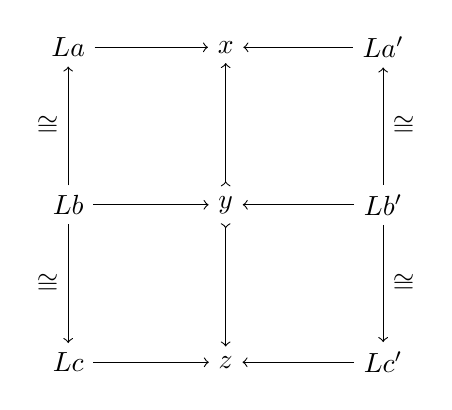
\begin{tikzpicture}
	\node (a) at (-1,1) {$ L a $};
	\node (x) at (1,1) {$ x $};
	\node (a') at (3,1) {$ L a' $};
	\node (b) at (-1,-1) {$ L b $};
	\node (y) at (1,-1) {$ y $};
	\node (b') at (3,-1) {$ L b' $};
	\node (c) at (-1,-3) {$ L c $};
	\node (z) at (1,-3) {$ z $};
	\node (c') at (3,-3) {$ L c' $};
	%
	\draw [->] (a) to (x);
	\draw [->] (a') to (x);
	\draw [->] (b) to (y);
	\draw [->] (b') to (y);
	\draw [->] (c) to (z);
	\draw [->] (c') to (z);
	\draw [->] (b) to node [left] {$ \cong $} (a);
	\draw [->] (b) to node [left] {$ \cong $} (c);
	\draw [>->] (y) to (x);
	\draw [>->] (y) to (z);
	\draw [->] (b') to node [right] {$ \cong $} (a');
	\draw [->] (b') to node [right] {$ \cong $} (c');
	\end{tikzpicture}
	\]
	where the arrows marked ``$ \rightarrowtail $'' are monic. 
\end{df}

\begin{df} \label{df_mon-rewrite-dble-cat}
	Denote by $ \MMonRewrite{L} $ the double category with $ \A $-objects as 0-cells, spans in $ \A $ whose legs are isomorphisms as vertical 1-cells, $ L $-open objects as horizontal 1-cells, and commuting diagrams in $ \X $ of form	
	\[
	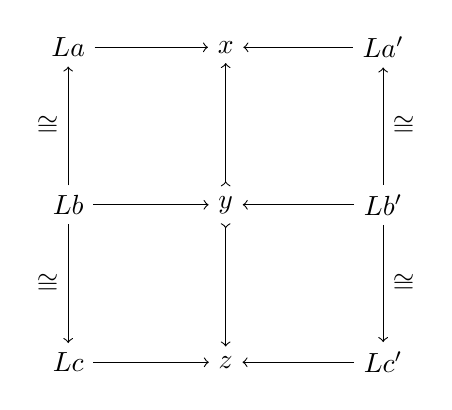
\begin{tikzpicture}
	\node (a) at (-1,1) {$ L a $};
	\node (x) at (1,1) {$ x $};
	\node (a') at (3,1) {$ L a' $};
	\node (b) at (-1,-1) {$ L b $};
	\node (y) at (1,-1) {$ y $};
	\node (b') at (3,-1) {$ L b' $};
	\node (c) at (-1,-3) {$ L c $};
	\node (z) at (1,-3) {$ z $};
	\node (c') at (3,-3) {$ L c' $};
	%
	\draw [->] (a) to (x);
	\draw [->] (a') to (x);
	\draw [->] (b) to (y);
	\draw [->] (b') to (y);
	\draw [->] (c) to (z);
	\draw [->] (c') to (z);
	\draw [->] (b) to node [left] {$ \cong $} (a);
	\draw [->] (b) to node [left] {$ \cong $} (c);
	\draw [>->] (y) to (x);
	\draw [>->] (y) to (z);
	\draw [->] (b') to node [right] {$ \cong $} (a');
	\draw [->] (b') to node [right] {$ \cong $} (c');
	\end{tikzpicture}
	\]
\end{df}

\begin{thm} \label{thm_mon-rewrite-isofibrant}
	The double category $ \MMonRewrite{L} $ is isofibrant.
\end{thm}

\begin{thm} \label{thm_mon-rewrite-dble-cat-smc}
	Let $ (\A, \otimes_{ \A }, I_{ \A }) $ and $ (\X, \otimes_{\X}, I_{\X}) $ be symmetric monoidal categories where $ \A $ has pullbacks and $ \X $ is a topos. Let $ L \from (\A, \otimes_{ \A }, I_{ \A }) \to (\X, \otimes_{\X}, I_{\X}) $ be a pullback preserving functor. Then $ (\MMonRewrite{L} , \otimes , I) $ is a symmetric monoidal double category with $ \otimes $ defined by
	\[
	\left( L a \to x \gets L b \right) \otimes
	\left( L c \to y \gets L d	\right) \coloneqq
	L (a \otimes_{\A} c) \to 
	x \otimes_{\X} y \gets L (b \otimes_{\A} d)
	\]
	and $ I $ by
	\[
	I \coloneqq ( L I_{\A} \to I_{\X} \gets L I_{\X} ).
	\]
\end{thm}

\begin{thm} \label{thm_mon-rewrite-cat-compact-closed}
	Let $ (\A, \otimes_{ \A }, I_{ \A }) $ and $ (\X, \otimes_{\X}, I_{\X}) $ be symmetric monoidal categories where $ \A $ has pullbacks and $ \X $ is a topos. Let $ L \from (\A, \otimes_{ \A }, I_{ \A }) \to (\X, \otimes_{\X}) $ be an adjunction where $ L $ preserves pullbacks.
	
	The horizontal edge bicategory $ \MonRewrite{L} \coloneqq  \mathcal{H} \left( \MMonRewrite{L} \right) $ in the sense of Shulman is symmetric monoidal.  Moreover, if the monoidal products $ \otimes_{\A} $ and $ \otimes_{\X} $ are coproducts, then the symmetric monoidal bicategory $ \MonRewrite{L} $ is compact closed.
\end{thm}


\begin{thm}
	Suppose each element from a grammar $ \Gamma $ in $ \StrCsp{L} $ is of the form 
	\[
	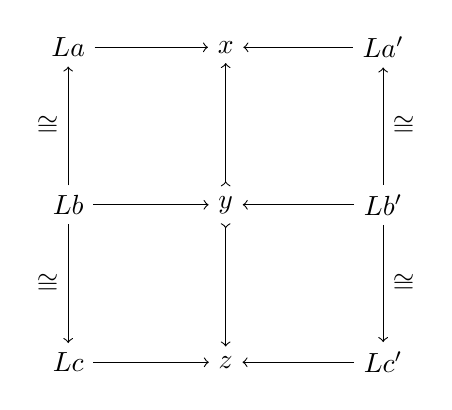
\begin{tikzpicture}
	\node (a) at (-1,1) {$ L a $};
	\node (x) at (1,1) {$ x $};
	\node (a') at (3,1) {$ L a' $};
	\node (b) at (-1,-1) {$ L b $};
	\node (y) at (1,-1) {$ y $};
	\node (b') at (3,-1) {$ L b' $};
	\node (c) at (-1,-3) {$ L c $};
	\node (z) at (1,-3) {$ z $};
	\node (c') at (3,-3) {$ L c' $};
	%
	\draw [->] (a) to (x);
	\draw [->] (a') to (x);
	\draw [->] (b) to (y);
	\draw [->] (b') to (y);
	\draw [->] (c) to (z);
	\draw [->] (c') to (z);
	\draw [->] (b) to node [left] {$ \cong $} (a);
	\draw [->] (b) to node [left] {$ \cong $} (c);
	\draw [>->] (y) to (x);
	\draw [>->] (y) to (z);
	\draw [->] (b') to node [right] {$ \cong $} (a');
	\draw [->] (b') to node [right] {$ \cong $} (c');
	\end{tikzpicture}
	\]
	then $ \Gamma $ generates a sub-double category $ \langle \langle \Gamma \rangle \rangle $ of $ \MMonRewrite{L} $.  The recipe is get the language $ \mathcal{L}(\Gamma)  \subseteq \Sp{\StrCsp{L}} $. Form the category as described in Definition \ref{df:ArrCatMonRwrt} from $ \mathcal{L}(\Gamma) $. Pair this, as an arrow category, with the object category $ \core{\Sp{\A}} $.
\end{thm}

\begin{thm}
	Same as above with monics thrown in.
\end{thm}










\end{document}